% ==============================
\section{Using the template}
% ==============================

This is a different section. You can write directly to the main.tex file, or write your document to these auxiliary files, it's up to you. You can create multiple new files if you want, it is more convenient for me to have one file for each section.

\subsection{Cite using Biblatex}

The Biblatex package has been loaded into the document, this package provides advanced bibliographic facilities for use with LaTeX. There are multiple ways of loading and use this package, so I recommend to read the documentation for advanced users. Below are shown some of the citation options:

\begin{itemize}
    \item \verb+\cite{Raghavan2007}+ produces \cite{Raghavan2007}
    \item \verb+\citep{Lou2013}+ produces \citep{Lou2013}
    \item \verb+\citeauthor{Newman2004}+ changes if the number of authors is too low: \citeauthor{Newman2004}
    \item \verb+\citeyear{Sobolevsky2014}+ produces \citeyear{Sobolevsky2014}
\end{itemize}

You should consider that the configuration in which the package was loaded will affect what each command prints.

\subsection{Insert figures, tables and equations}

Below are some basic examples for inserting different content into the manuscript. Note that the configuration with which a figure or table is inserted will define where it is located.

\subsubsection{Figures}

An image file is provided, so that you can see an example of image insertion.

\begin{figure}[htb]
    \centering
    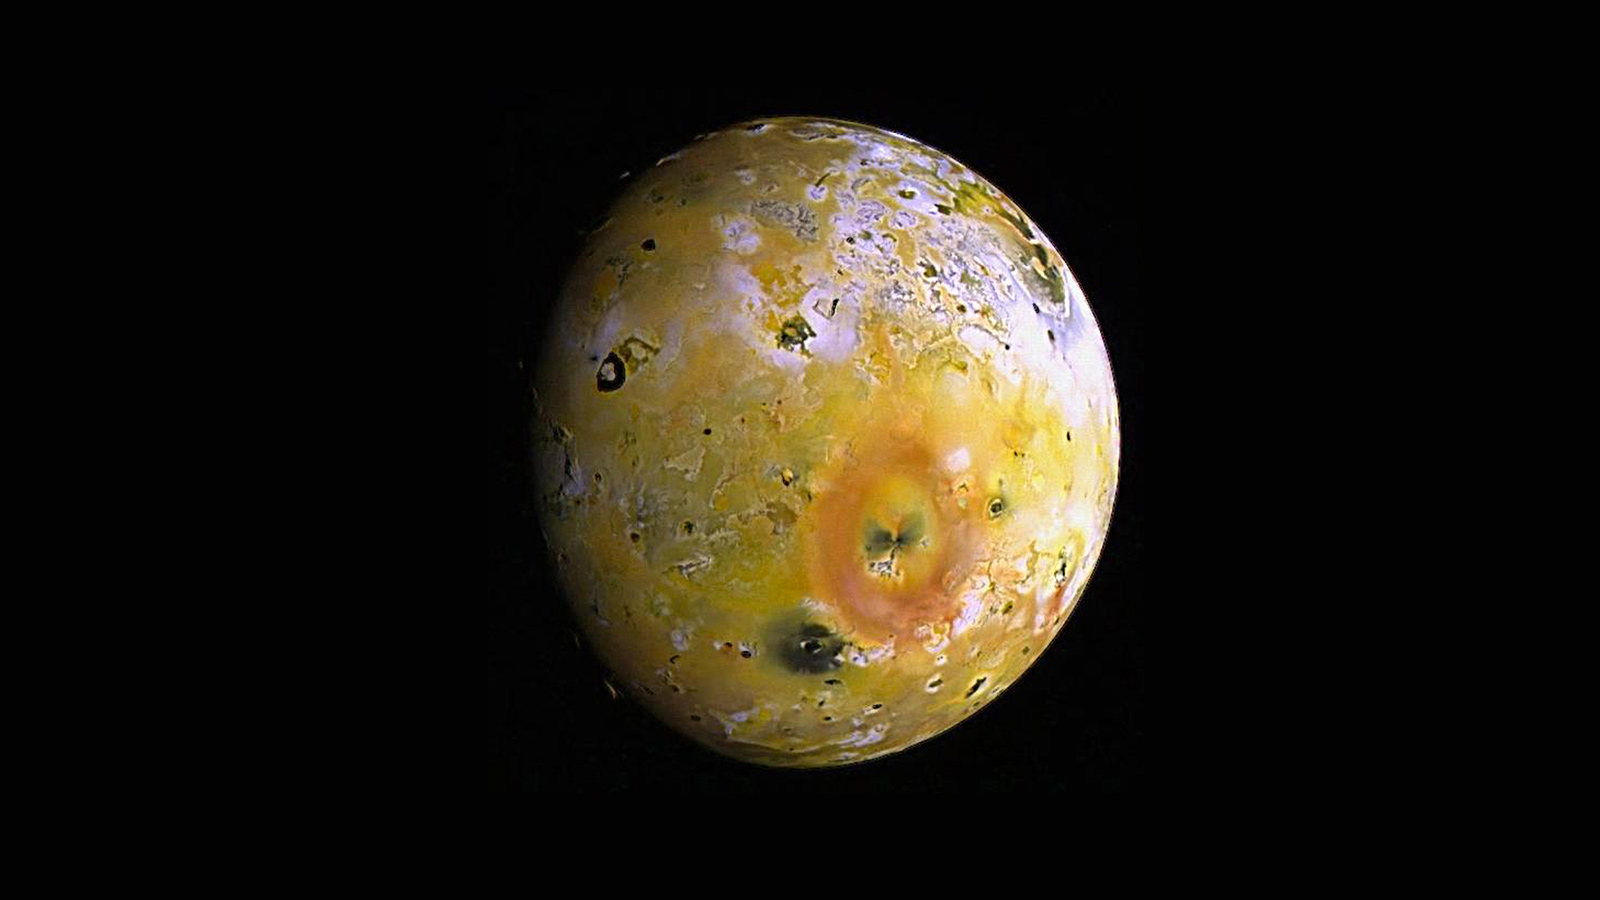
\includegraphics[width=0.8\columnwidth]{img/io_moon.jpg}
    \caption{Io is the innermost and third-largest of the four Galilean moons of the planet Jupiter.}
    \label{fig:my_label}
\end{figure}

If you change the environment into \verb+\begin{figure*}+ \verb+...+ \verb+\end{figure*}+ you will get a single column figure inserted.

\subsubsection{Tables}

There are a variety of ways to insert tables in Latex, so only one way will be exemplified that allows them to look similar to manuscripts.

First of all, we have the Table \ref{tab:population}. This is how a table would be written to use the width of the column and delete the extra space on the sides.

\begin{table}[htb]
    \caption{Countries with the largest population in the world.}
    \label{tab:population}
    \begin{tabular*}{\columnwidth}{@{\extracolsep{\fill}} *{2}{l} r @{}}
        \toprule
        \# & Country & Population (2020) \\
        \midrule
        1 & China & 1,439,323,776 \\
        2 & India & 1,380,004,385 \\
        3 & United States & 331,002,651 \\
        4 & Indonesia & 273,523,615 \\
        5 & Pakistan & 220,892,340 \\
        \bottomrule
    \end{tabular*}
\end{table}

Of course, there are cases where our tables contain too much information, so it is not possible to adapt them to the width of a column. In those cases we can create a table with the width of all the text, as seen in Table \ref{tab:extended_population}. Furthermore, I have defined the \verb+\tablenote+ command to add footnotes to tables.

\begin{table*}[htb]
    \caption{Countries with the largest population, but with more data.}
    \label{tab:extended_population}
    \begin{tabular*}{\textwidth}{@{\extracolsep{\fill}} *{6}{l} @{}}
    \toprule
        \# & Country & Population (2020) & Yearly change & Net change & Density ($n/km^2$)\\
        \midrule
        1 & China & 1,439,323,776 & 0.39\% & 5,540,090 & 153 \\
        2 & India & 1,380,004,385 & 0.99\% & 13,586,631 & 464 \\
        3 & United States & 331,002,651 & 0.59\% & 1,937,734 & 36 \\
        4 & Indonesia & 273,523,615 & 1.07\% & 2,898,047 & 151 \\
        5 & Pakistan & 220,892,340 & 2.00\% & 4,327,022 & 287 \\
        \bottomrule
    \end{tabular*}
    \tablenote{Source: United Nations, Department of Economic and Social Affairs, Population Division. \href{https://esa.un.org/unpd/wpp/}{World Population Prospects: The 2019 Revision.} (Medium-fertility variant).}
\end{table*}

\subsubsection{Equations}

We can easily insert equations using the environment \verb+\begin{equation} ... \end{equation}+. Equations inserted through this environment are automatically numbered. For example we can write the heat equation.

\begin{equation}
    \frac{\partial u}{\partial t} = \alpha \Delta u
\end{equation}

On the other hand we can write this function in Cartesian coordinates, assuming $u(x,y,z,t)$ as solution of the equation.

\begin{equation}
    \frac{\partial u}{\partial t} = \alpha \left( \frac{\partial^2 u}{\partial x^2} + \frac{\partial^2 u}{\partial y^2} + \frac{\partial^2 u}{\partial z^2} \right)
    \label{eq.2}
\end{equation}

You can the reference this equations if you add them a label using \verb+\ref{eq.2}+ and this will gives you the number of the equation (\ref{eq.2}).